\clearpage
\section{Campaña final de optimización}

Esta sección incorpora la campaña controlada ejecutada después de las dos baterías históricas. Su propósito fue comprobar qué cambios reducen el coste de comunicación observado en la corrida de 906 s y separar tres efectos que antes estaban mezclados: el algoritmo de difusión, la topología de la partición y el tamaño del problema.

\subsection{Protocolo y control de calidad}

Las matrices usan el kernel \texttt{tiled} con bloque 64, afinidad de un proceso por núcleo y las interfaces de red fijadas en el lanzador. La variante \texttt{1d} distribuye filas de $A$, realiza una difusión global de $B$ y reúne $C$. La variante \texttt{1d-hier} primero difunde entre un líder por nodo y después dentro de cada nodo. SUMMA 2D se evalúa solo con $P=64$, porque la implementación exige una malla cuadrada. El microbenchmark de Bcast transmite una matriz de 75.497 MB y comprueba una huella de 64 bits idéntica en todos los procesos.

Se conservaron 118 intentos válidos: cinco repeticiones para las comparaciones principales de $N=3072$ y tres para tamaños mayores, trapecio y difusión aislada. El auditor contrasta cada fila del CSV con su log, comprueba las sumas de control de matrices, verifica el error numérico del trapecio y genera \texttt{SHA256SUMS}. Los intentos piloto y de humo se mantienen en el repositorio como validación operativa, pero no entran en las medianas de esta sección.

\begin{landscape}\footnotesize\renewcommand{\arraystretch}{1.0}
\input{tablas_optimizacion}
\end{landscape}

\subsection{Resultados principales}

\begin{figure}[htbp]
\centering
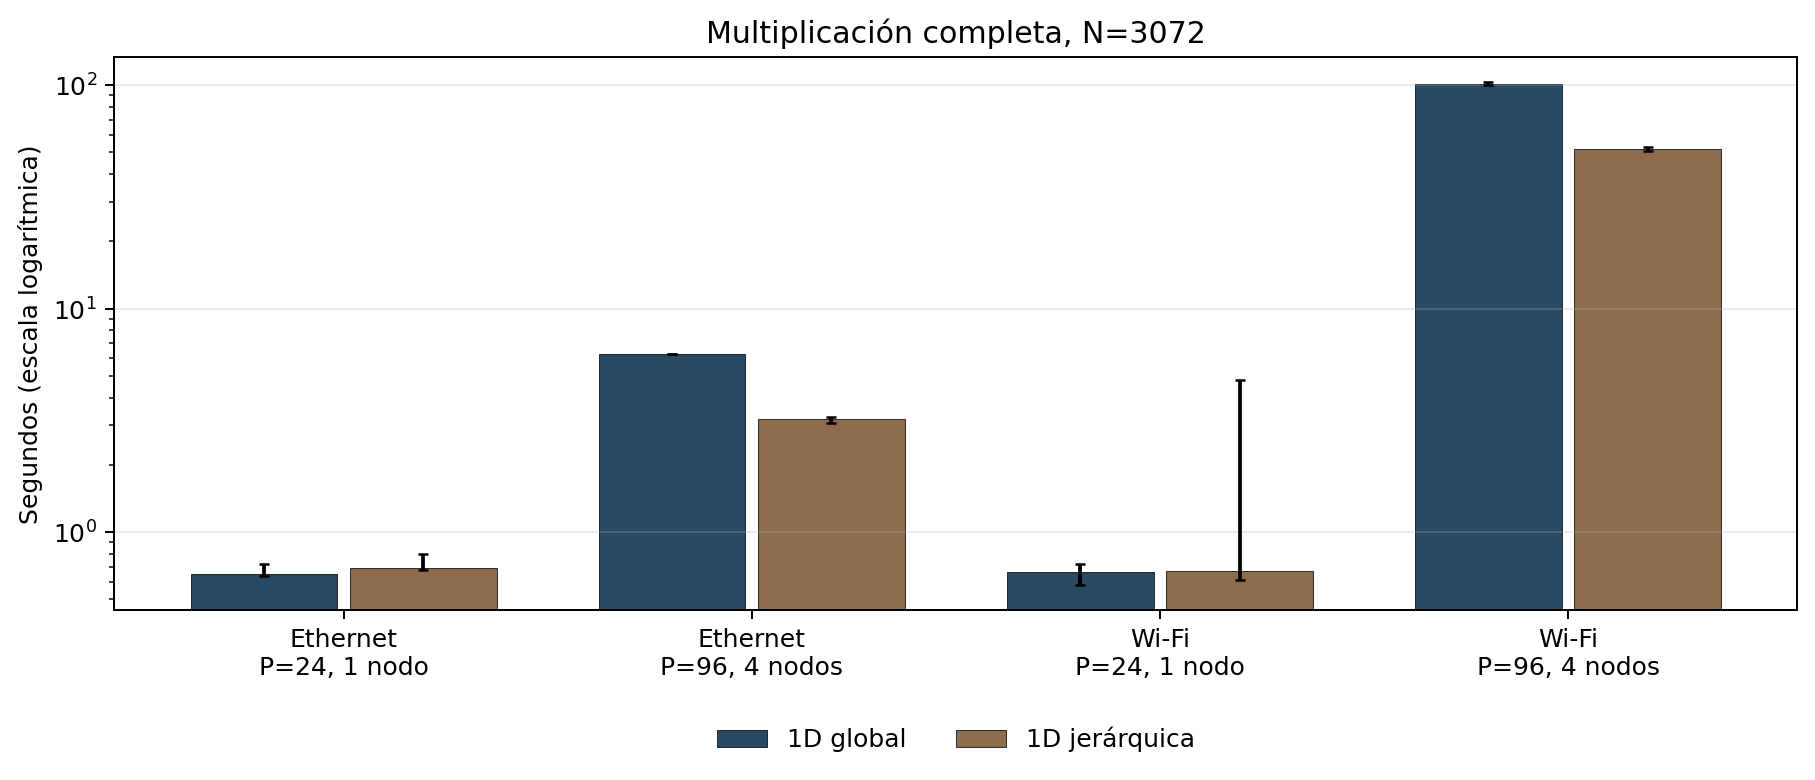
\includegraphics[width=0.94\linewidth]{img/optimizacion_matrices.png}
\caption{Multiplicación completa para $N=3072$. Se muestran medianas y rangos de las repeticiones válidas; la escala vertical es logarítmica.}
\end{figure}

\begin{figure}[htbp]
\centering
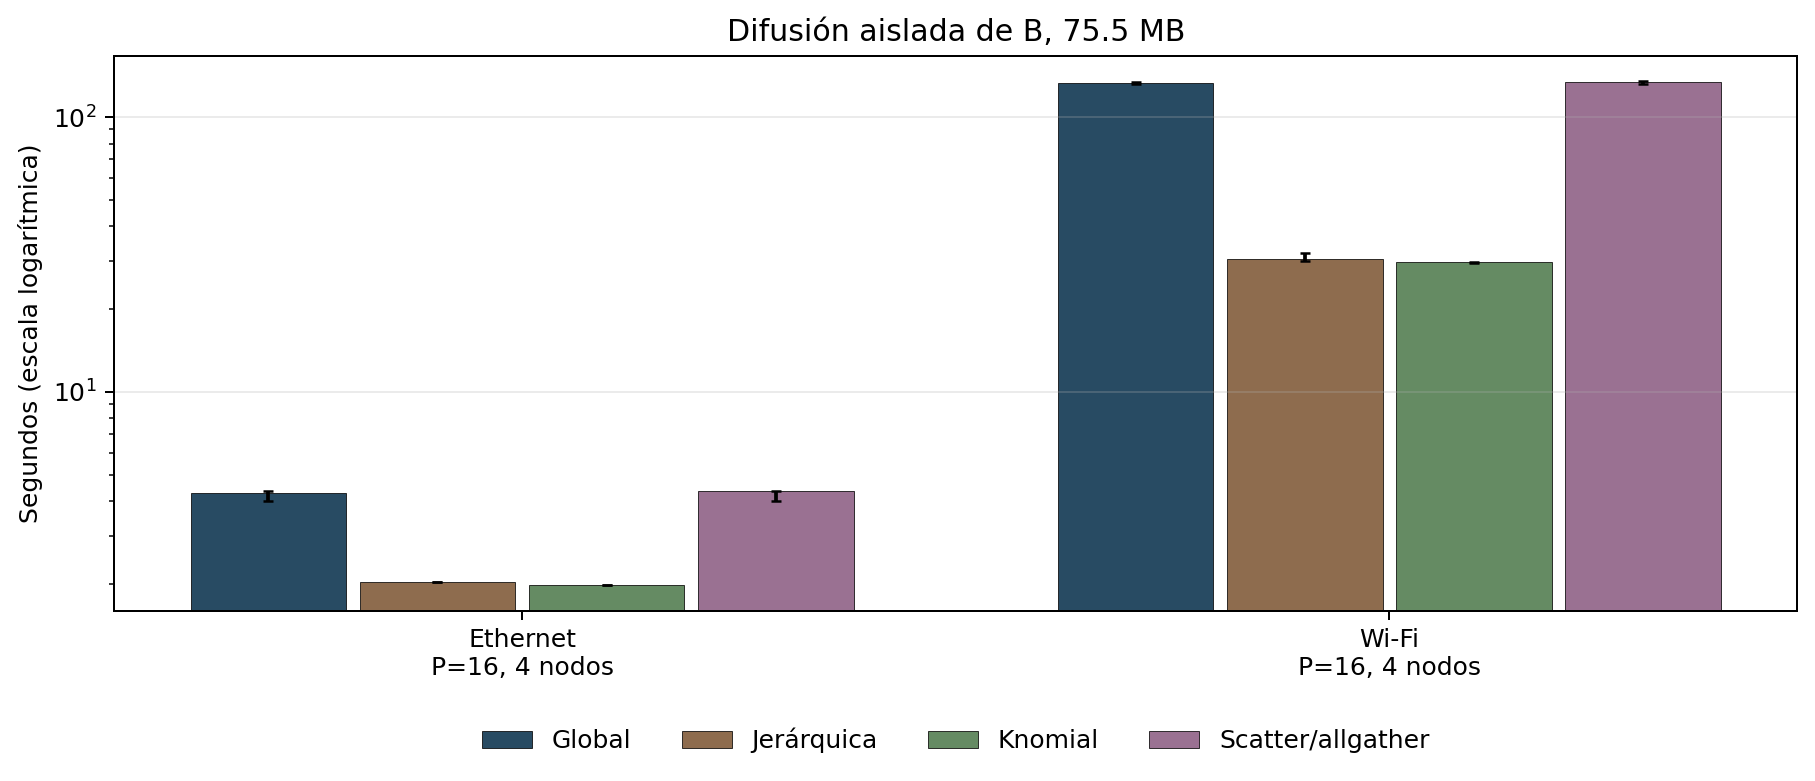
\includegraphics[width=0.82\linewidth]{img/optimizacion_bcast.png}
\caption{Difusión aislada de $B$ con 16 procesos. Las barras comparan la colectiva global, la jerárquica y dos selecciones del componente \texttt{tuned}.}
\end{figure}

\begin{figure}[htbp]
\centering
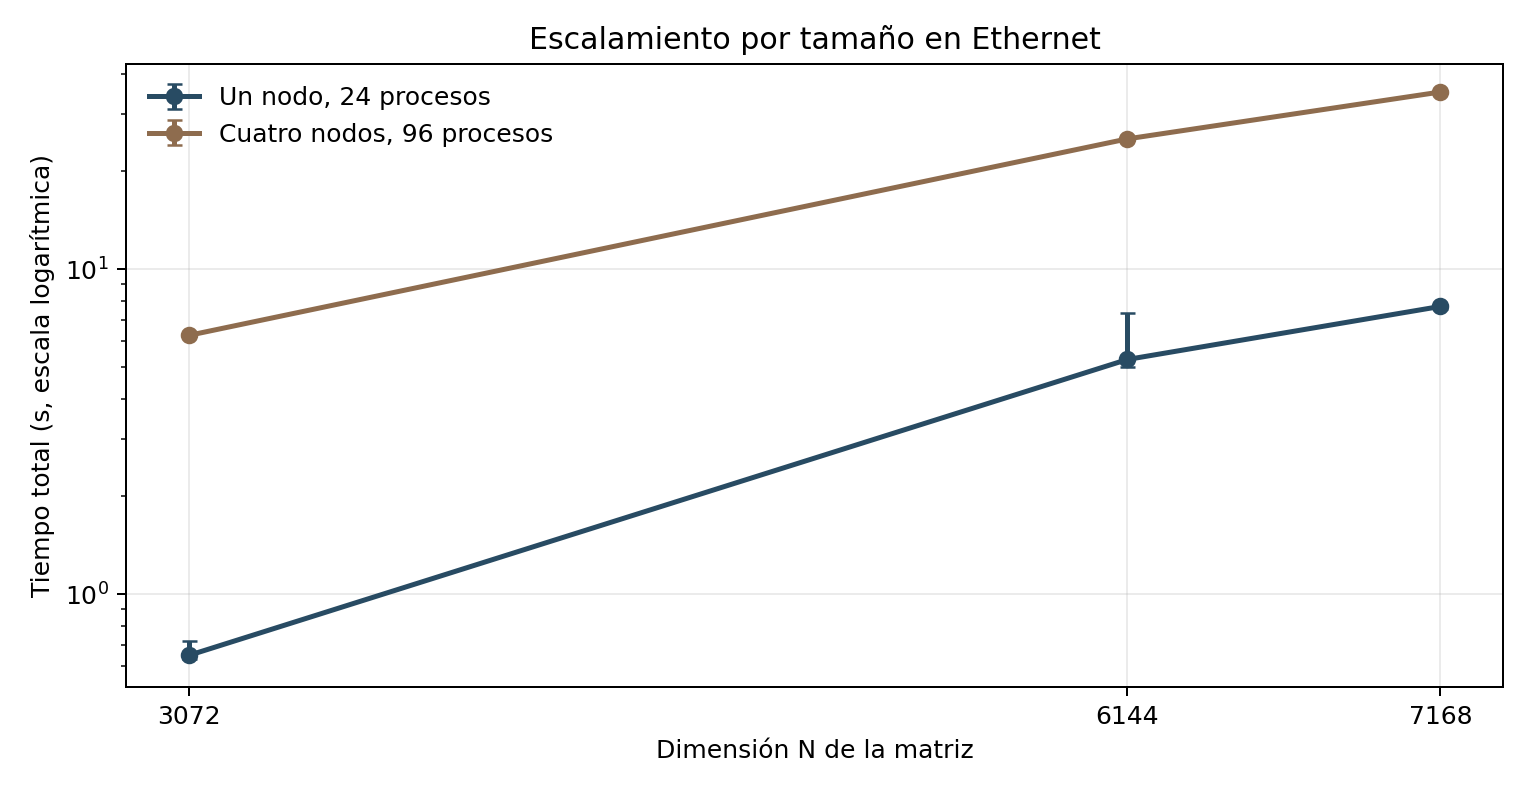
\includegraphics[width=0.78\linewidth]{img/optimizacion_tamano.png}
\caption{Escalamiento por tamaño en Ethernet. Cada punto es la mediana y las barras muestran el rango observado.}
\end{figure}

\subsection{Qué mejoras sí quedaron demostradas}

En Ethernet, la difusión jerárquica explícita frente a 1D por defecto a $P=96$ dio un cociente de tiempos 1.95\,veces y un cociente de TX agregados 2.11\,veces. Un valor mayor que 1 favorece la variante jerárquica. El máximo de la fase Bcast pasó de 5.611 a 2.474 s.


En Wi-Fi, la difusión jerárquica explícita frente a 1D por defecto a $P=96$ dio un cociente de tiempos 1.96\,veces y un cociente de TX agregados 2.13\,veces. Un valor mayor que 1 favorece la variante jerárquica. El máximo de la fase Bcast pasó de 88.904 a 40.272 s.


En Ethernet, 1D frente a SUMMA 2D, ambos con $P=64$, dio un cociente de tiempos 0.57\,veces y un cociente de TX agregados 0.53\,veces. Un valor menor que 1 favorece 1D.


En Wi-Fi, 1D frente a SUMMA 2D, ambos con $P=64$, dio un cociente de tiempos 0.59\,veces y un cociente de TX agregados 0.51\,veces. Un valor menor que 1 favorece 1D.


En la difusión aislada por Ethernet, la colectiva global frente a la jerárquica dio un cociente de tiempo 2.11\,veces y de TX agregado 4.33\,veces.


En la difusión aislada por Wi-Fi, la colectiva global frente a la jerárquica dio un cociente de tiempo 4.37\,veces y de TX agregado 4.41\,veces.


Con 16 procesos y difusión global por Ethernet, cuatro nodos frente a uno dieron un cociente 37.08\,veces.


En Ethernet, cuatro nodos con 96 procesos frente a un nodo con 24 procesos dieron un cociente $T_{96}/T_{24}$ de 9.65\,veces. Aquí un valor mayor que 1 favorece un nodo.


En Wi-Fi, cuatro nodos con 96 procesos frente a un nodo con 24 procesos dieron un cociente $T_{96}/T_{24}$ de 151.70\,veces. Aquí un valor mayor que 1 favorece un nodo.


Para $N=6144$ por Ethernet, $T_{96}/T_{24}$ fue 4.77\,veces.


Para $N=7168$ por Ethernet, $T_{96}/T_{24}$ fue 4.57\,veces.


Trapecio con $n=10^8$ y $P=24$: $T_{sim}/T_{asim}$ fue 1.70\,veces.


Trapecio con $n=10^8$ y $P=96$: $T_{sim}/T_{asim}$ fue 1.07\,veces.


Trapecio con $n=10^{11}$ y $P=24$: $T_{sim}/T_{asim}$ fue 1.05\,veces.


Trapecio con $n=10^{11}$ y $P=96$: $T_{sim}/T_{asim}$ fue 0.97\,veces.



La comparación de matrices es especialmente informativa porque conserva el cálculo local y cambia el transporte de $B$. Con cuatro nodos, la variante jerárquica reduce aproximadamente a la mitad el tiempo total y el TX agregado en las dos redes. El microbenchmark reproduce la dirección del efecto sin el ruido del cálculo: la razón global/jerárquica es 2.11 por Ethernet y 4.37 por Wi-Fi, mientras el cociente de TX es 4.33 y 4.41.

\subsection{Resultados que no deben sobreinterpretarse}

El hecho de que \texttt{1d-hier} sea más rápido no demuestra que la colectiva global anterior enviara exactamente una copia por proceso ni que todo el tráfico local viajara por TCP. Cada proceso sigue reservando su propia copia completa de $B$; la variante nueva cambia el patrón de mensajes, no convierte todavía la memoria en una ventana compartida. Para identificar el algoritmo interno de Open MPI habría que registrar el componente colectivo seleccionado o ejecutar un barrido controlado de MCA.

La suma TX de los nodos y el contador TX+RX del servidor de las baterías anteriores tienen alcances diferentes. Se conservan ambos porque responden preguntas distintas: el primero permite comparar la presión agregada en la campaña nueva y el segundo documenta qué observó una interfaz concreta durante la batería ampliada. Ninguna de las dos cifras equivale al volumen útil exacto de una colectiva.

\subsection{Implicaciones prácticas}

Para repetir el mejor resultado medido con matrices, conviene empezar con 24 procesos en un nodo. Si se necesita usar los cuatro nodos, la primera opción probada es la difusión jerárquica explícita. La partición 2D debe rediseñarse antes de escalarla a 96 procesos: la versión actual no acepta una malla rectangular y su coste completo fue mayor que 1D en $P=64$. Para trabajos de trapecio suficientemente grandes, sí conviene usar los 96 procesos; el beneficio proviene de tener mucho cálculo por cada reducción de un escalar.

\begin{idea}
La recomendación que sobrevive a todos los datos es medir por separado cálculo y comunicación. El tamaño del mensaje, la red y el número de procesos cambian la decisión más que el nombre del algoritmo. En este clúster, la reducción de copias entre nodos produjo la mejora más grande y reproducible para matrices.
\end{idea}

